\begin{frame}
  \frametitle{Performance Evaluation}
 Through simulations the following two metrics for various values of $\Delta$ were evaluated:
  \begin{itemize}
  \item Time taken for 10\% of a large database to become semantically corrupt
    \item Fraction of transactions aborted per second
  \end{itemize}
\end{frame}

\begin{frame}
  \frametitle{Time until 10\% semantic corruption $\boldsymbol{log(U)}$ vs Transaction Arrival Rate $(\boldsymbol{\lambda})$}
  \begin{center}
    For $\Delta = 50ms$, time taken for 10\% of a large database to become semantically corrupt is between to $1$-$75$ years
  \end{center}
    \begin{figure}[h!]
    \centering
    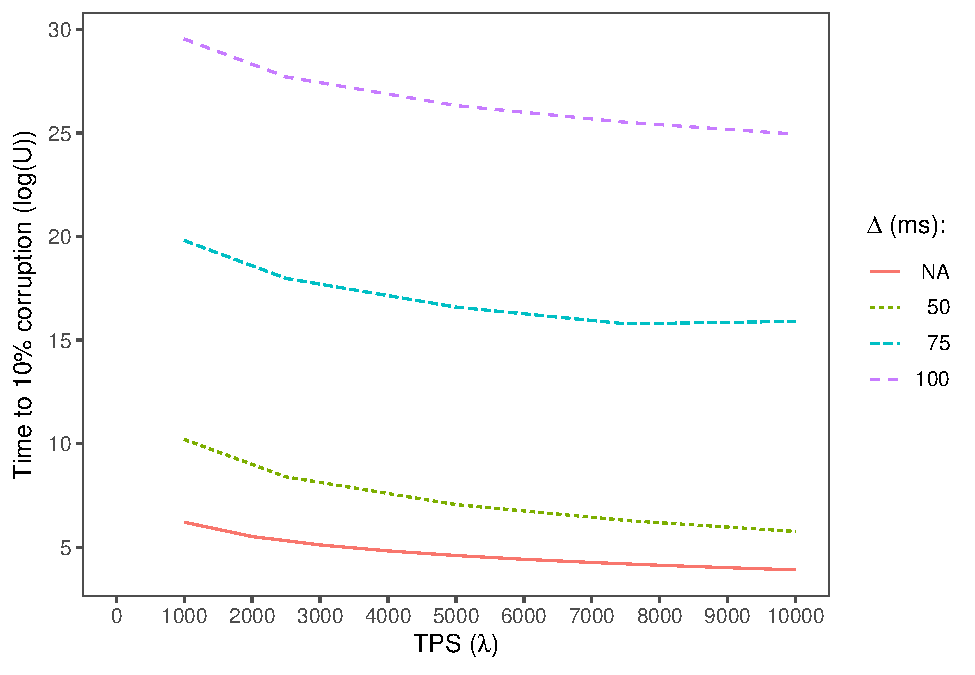
\includegraphics[scale=0.5]{./figures/delta}
  \end{figure}
\end{frame}

\begin{frame}
  \frametitle{Fraction of Aborts $(\boldsymbol{\alpha})$ vs Transaction Arrival Rate $(\boldsymbol{\lambda})$}
  \begin{center}
    For $\Delta = 50 ms$, the fraction of aborts is between 1 − 5\%
  \end{center}
    \begin{figure}[h!]
    \centering
    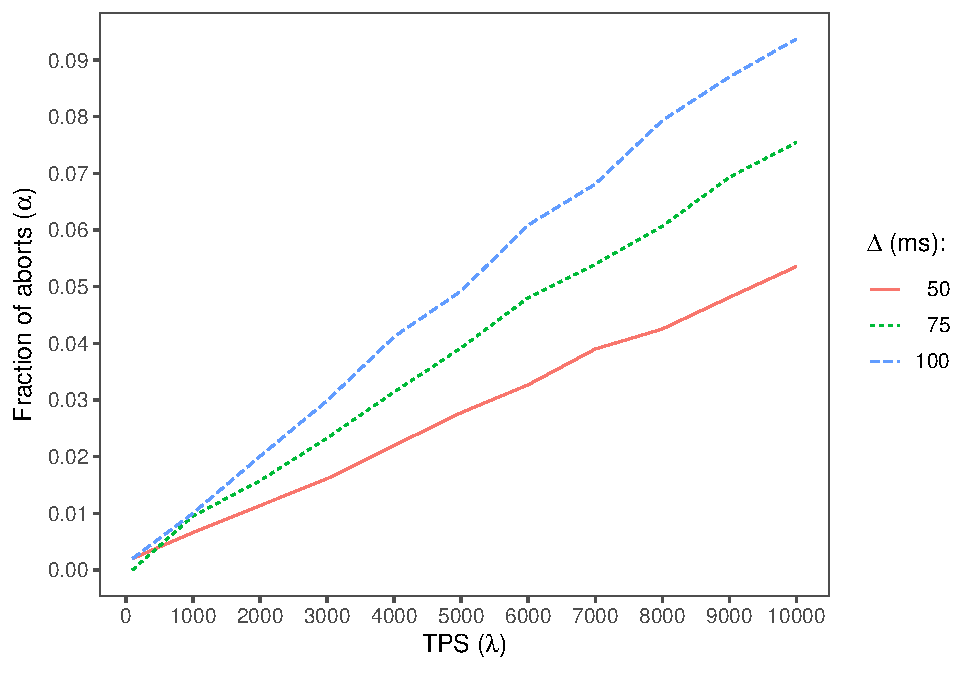
\includegraphics[scale=0.5]{./figures/aborts}
  \end{figure}
\end{frame}